


\chapter{Economic Design Optimisation}
\label{ch: economical design optimisation }

In the hydrodynamic analysis, it was sometimes hard to judge which configuration could be labelled as best performing because the mean wave drift force and transmitted wave height possess different units; Newtons and metres. A cost function is created to convert these responses to the same quantity, namely: euros. The costs of the construction of the breakwater should be less than the cost reduction on the mooring system of the floating island due to the presence of this breakwater. Therefore, an economic design optimisation is performed. How both the mean wave drift force and wave transmission are implemented in the economical optimisation is thoroughly explained in Section \ref{sec: cost analysis methodology }. The approach is discussed in Section \ref{sec: approach costs DI1 H3 captive}, the correlation of factors with respect to responses in Section \ref{sec: correlation costs DI1 H3 captive} and the design optima are announced in Section \ref{sec: design optima costs DI1 H3 captive}.

\section{{Design Iteration 1}}

\subsection{Approach}
\label{sec: approach costs DI1 H3 captive}

To make a fair comparison between the outcome of the hydrodynamic analysis and the economical analysis, the same design space as in Section \ref{sec: design iteration 1 captive} is used. Therefore, also the parameters boundaries are the same as in Table \ref{tab: boundaries DI1 captive}. The simulations done for this optimisation are done with Wave Condition 1: H = 3 metres and T = 6 seconds. 


\subsection{Correlation}
\label{sec: correlation costs DI1 H3 captive}

Figures \ref{fig: correlation costs DI1 H3 captive} and \ref{fig: perturbation R2 costs DI1 H3 captive} show that the total cost reduction has a strong negative correlation with factor B (the width of the breakwater). This is mainly due to the positive correlation between the floater width and the breakwater costs. The costs of the required mooring system of the breakwater alone (second response) are negatively correlated with the position of the waterline (i.e., submerged breakwaters require a cheaper mooring system than surfaced ones). 

% \begin{figure}[h]
%     \centering
%     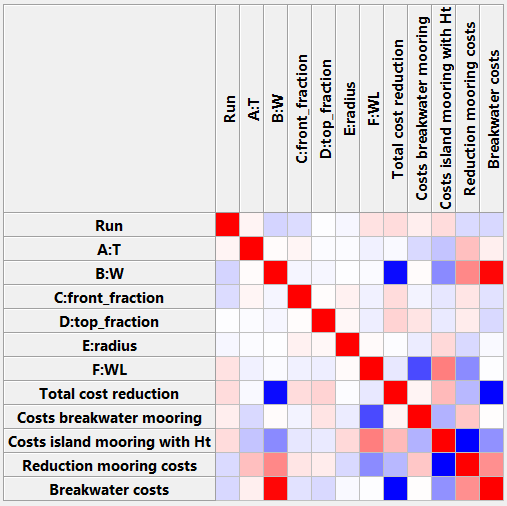
\includegraphics[width=0.3\linewidth]{figures/ComFLOW/Results DI1/costs/correlation_costs.png}
%     \caption{Correlation between factors and responses}
%     \label{fig: correlation costs DI1 H3 captive}
% \end{figure}

\begin{figure}[H]
    \centering
    \begin{subfigure}[b]{0.35\textwidth}
        \centering
        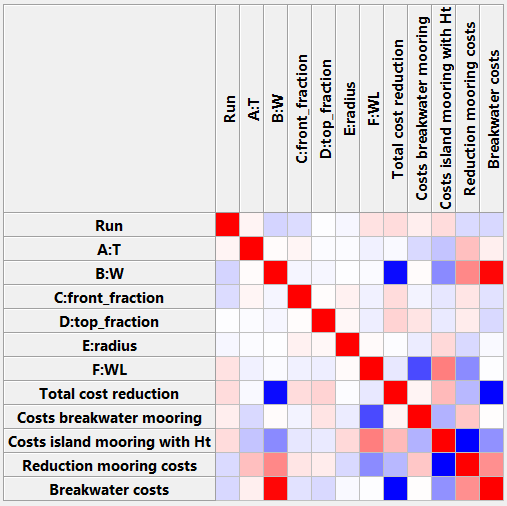
\includegraphics[width=\linewidth]{figures/ComFLOW/Results DI1/costs/correlation_costs.png}
        \caption[]%
        {{\small Correlation between factors and responses}}    
        \label{fig: correlation costs DI1 H3 captive}
    \end{subfigure}
    \hfill
    \begin{subfigure}[b]{0.49\textwidth}  
        \centering 
        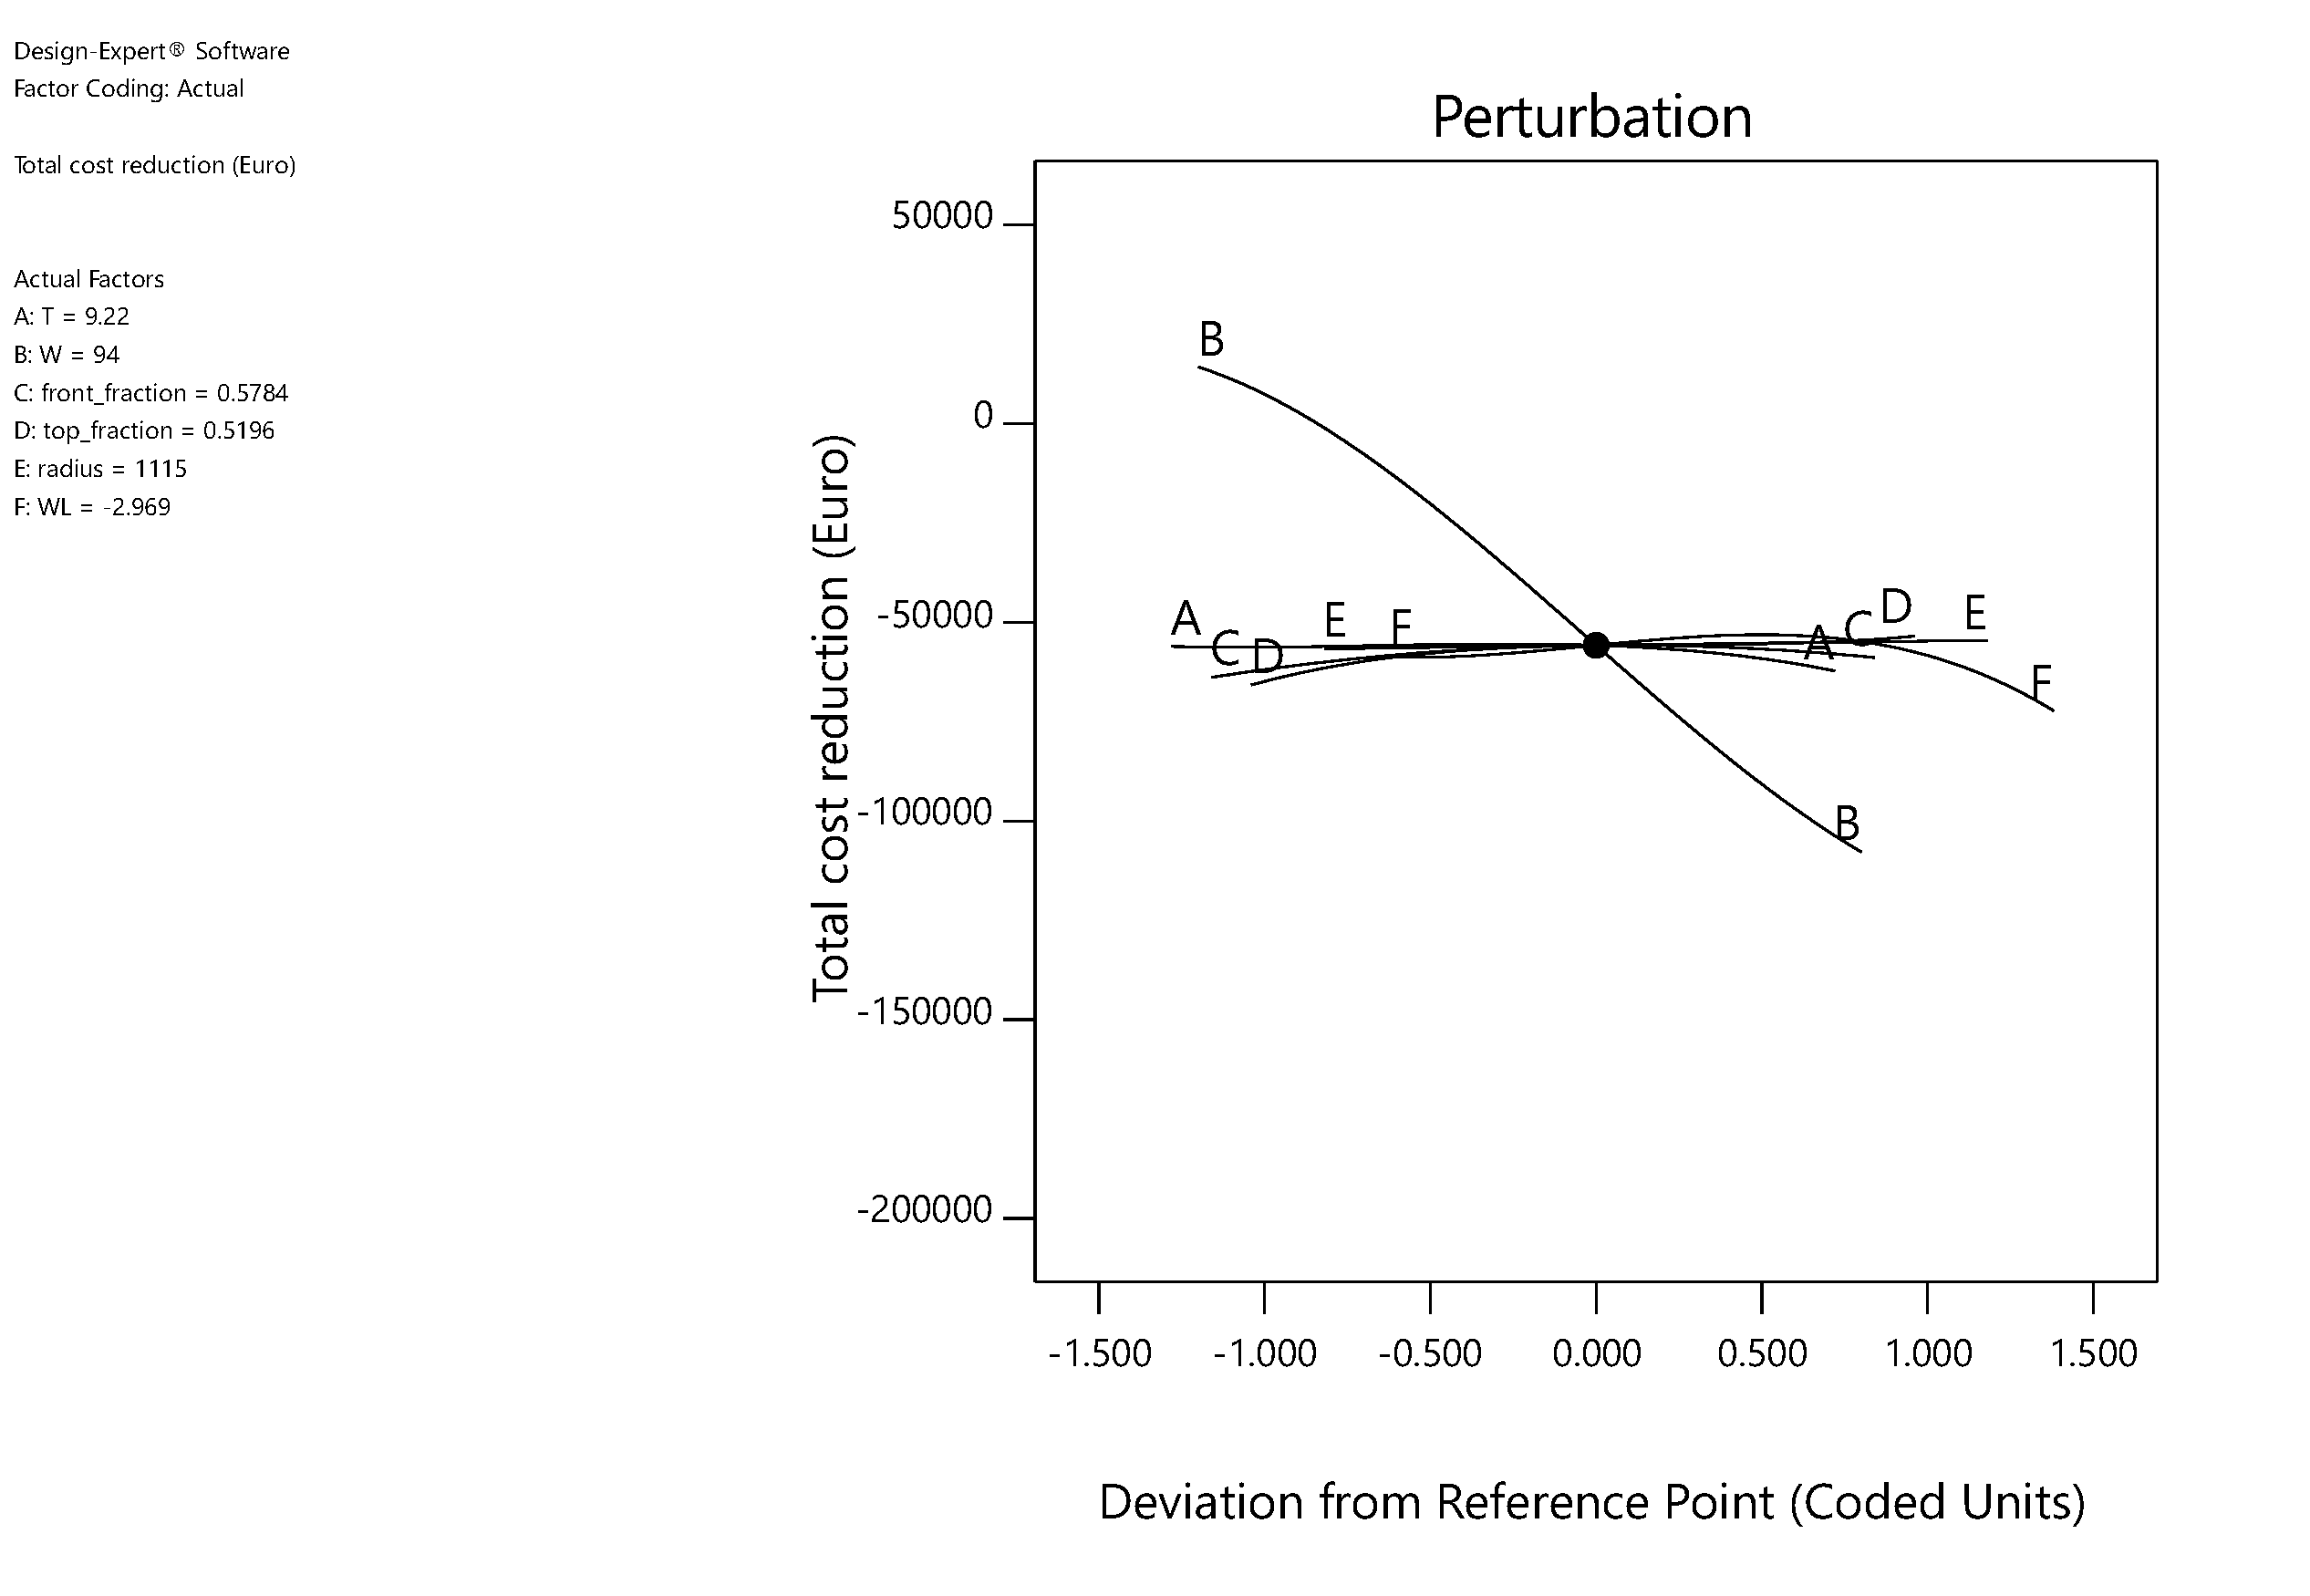
\includegraphics[width=\linewidth]{figures/ComFLOW/Results DI1/costs/Perturbation Total cost reduction.pdf}
        \caption[]%
        {{\small Perturbation Response: Total Cost Reduction}}    
        \label{fig: perturbation R2 costs DI1 H3 captive}
    \end{subfigure}


    \caption{}
    \label{fig: }
\end{figure}

Figure \ref{fig: Fd_norm_VS cost reduction mooring H3 DI1 captive} shows the correlation between the mean wave drift force experienced by the breakwaters with respect to their cost reduction of the required mooring system of both the breakwater and the floating island connected at the lee-side of the breakwater. Many breakwater are able to realise a cost reduction of the mooring system, even while experiencing large mean wave drift forces, because of their wave attenuating performance. But, most of the breakwaters breakwaters providing the most reduction in mooring cost are expensive themselves, which can also be observed in Figure \ref{fig:  geometrycosts vs cost reduction mooring H3 DI1 captive}. The only breakwaters resulting in positive total cost reductions are the orange and yellow ones in the top left corner of this plot. 


\begin{figure}[h]
    \centering
    \begin{subfigure}[b]{0.49\textwidth}
        \centering
        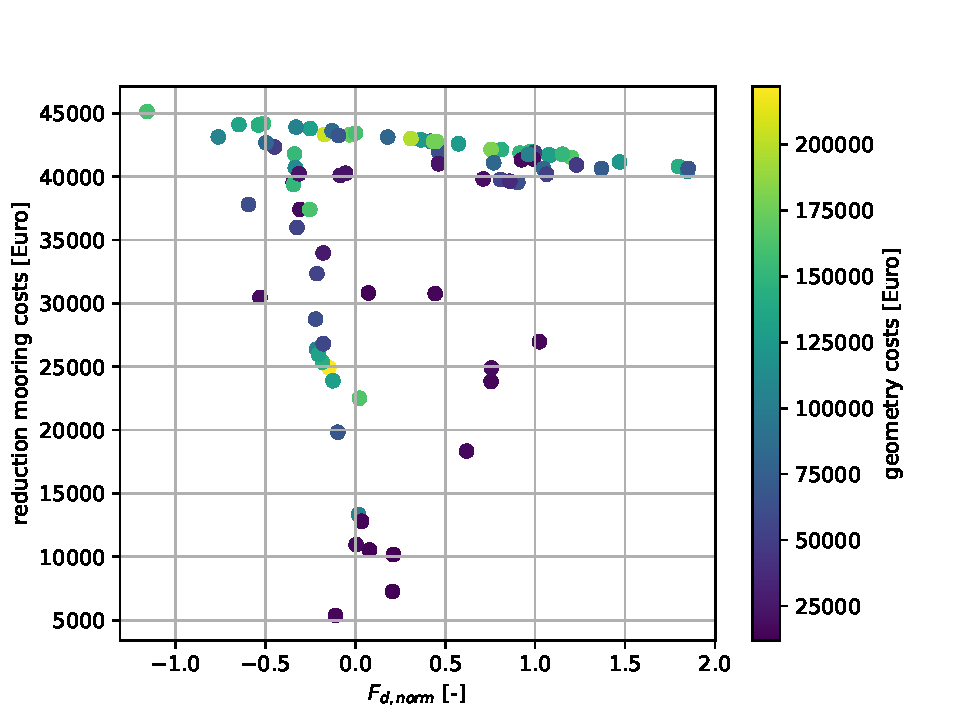
\includegraphics[width=\linewidth]{figures/ComFLOW/Results DI1/costs/Fd_norm_VS_cost_reduction_mooring.pdf}
        \caption[]%
        {{\small Mean wave drift force w.r.t. reduction island mooring costs}}    
        \label{fig: Fd_norm_VS cost reduction mooring H3 DI1 captive}
    \end{subfigure}
    \hfill
    \begin{subfigure}[b]{0.49\textwidth}  
        \centering 
        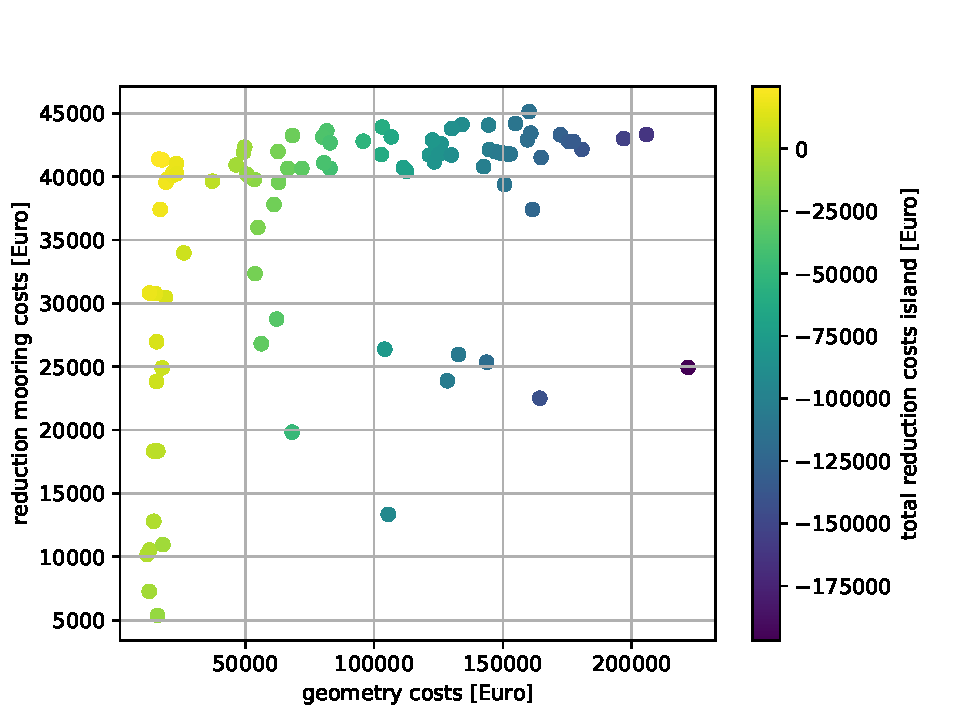
\includegraphics[width=\linewidth]{figures/ComFLOW/Results DI1/costs/geometrycosts_VS_cost_reduction_mooring.pdf}
        \caption[]%
        {{\small Geometry costs w.r.t. reduction island mooring costs}}    
        \label{fig:  geometrycosts vs cost reduction mooring H3 DI1 captive}
    \end{subfigure}
    
    \caption{Results of simulated breakwaters}
    \label{fig: }
\end{figure}



\subsection{Design Optima}
\label{sec: design optima costs DI1 H3 captive}

The design optima based on the costs are given in two variants. A box-type structure below the waterline and a breakwater with a sloping beach crossing the water surface. Both structures converged to the smallest width, 10 metres. The box-type structure has a depth of 2.7 metres and the other a relatively large depth of circa 8 metres. 

\begin{table}[h]
\centering
\scalebox{0.65}{
\begin{tabular}{@{}cccccccccccc@{}}
\toprule
configuration & T        & W        & front\_fraction & top\_fraction & radius   & WL & \texteuro$_{reduction}$ & \texteuro$_{mooring~bw}$  & \texteuro$_{mooring~island}$  & \texteuro$_{mooring reduction}$ & \texteuro$_{breakwater}$      \\ \midrule
1  & 8.50  & 10.00 & 0.01 & 0.56 & 1989.28 & -4.27 & 26529.26 & 1689.95 & 10924.95 & 37328.42 & 14809.65 \\
2  & 7.32  & 10.84 & 0.01 & 0.66 & 2000.00 & -5.68 & 26303.25 & 1150.72 & 17064.81 & 30539.70 & 13523.41 \\
3  & 9.49  & 10.00 & 0.01 & 0.72 & 1999.99 & -3.51 & 26119.39 & 1777.92 & 9564.75  & 38947.00 & 17393.69 \\
4  & 8.97  & 11.03 & 0.01 & 0.60 & 1999.99 & -2.40 & 26109.77 & 1282.55 & 7902.01  & 38517.55 & 17678.02 \\
5  & 2.66  & 10.05 & 0.99 & 0.99 & 500.11  & 0.49  & 26048.41 & -485.58 & 11448.89 & 34479.81 & 10825.75 \\
6  & 10.71 & 10.00 & 0.01 & 0.59 & 2000.00 & -2.04 & 26011.19 & 1427.57 & 6542.94  & 39991.51 & 19594.92 \\
7  & 8.90  & 10.00 & 0.01 & 0.80 & 1999.96 & -2.59 & 25754.30 & 1343.34 & 9665.31  & 37451.44 & 16585.14 \\
8  & 3.39  & 10.00 & 0.99 & 0.99 & 500.01  & 0.38  & 25737.49 & -250.50 & 11752.02 & 35330.83 & 11102.63 \\
9  & 10.15 & 10.05 & 0.04 & 0.57 & 2000.00 & -2.85 & 25727.60 & 1716.07 & 7248.75  & 40415.87 & 18135.08 \\
10 & 7.49  & 10.00 & 0.01 & 0.77 & 1987.01 & -2.00 & 25708.77 & 1000.37 & 11328.99 & 35876.85 & 14145.59 \\\bottomrule
\end{tabular}
}
\caption{Parameters optimal breakwaters based on costs}
\label{tab: params design iteration 1 captive costs 1to10}
\end{table}


\begin{figure}[h]
    \centering
    \begin{subfigure}[b]{0.475\textwidth}
        \centering
        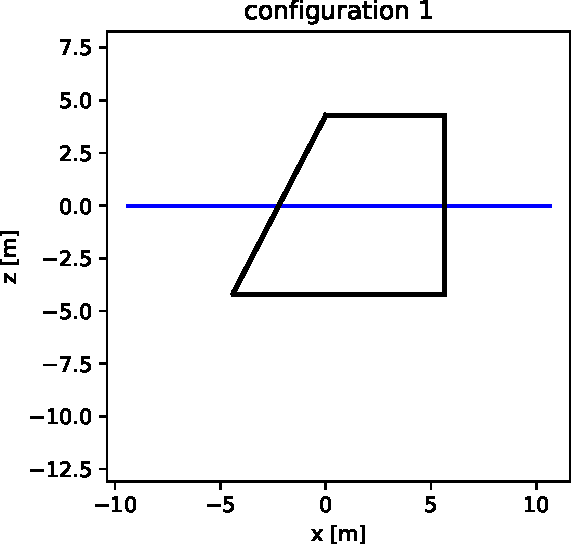
\includegraphics[width=\textwidth]{figures/ComFLOW/Breakwater Geometries/Design Iteration 1 captive/top from costs/breakwater_geometry1.pdf}
        \caption[]%
        {{\small}}    
        \label{fig: opt breakwater 1 costs DI1}
    \end{subfigure}
    \hfill
    \begin{subfigure}[b]{0.475\textwidth}  
        \centering 
        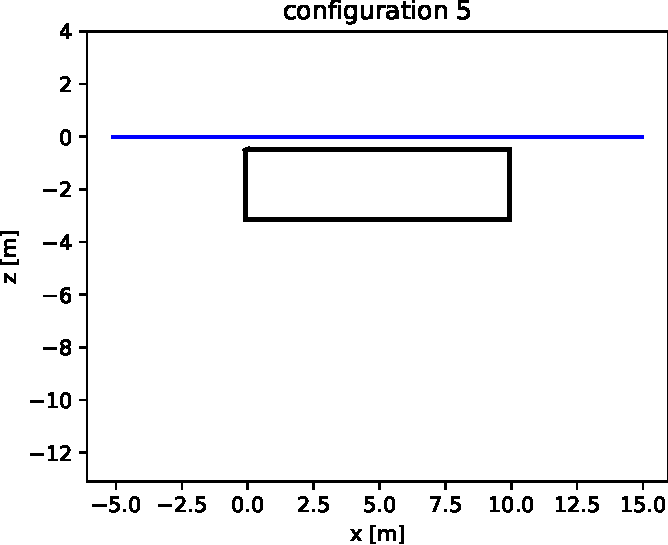
\includegraphics[width=\textwidth]{figures/ComFLOW/Breakwater Geometries/Design Iteration 1 captive/top from costs/breakwater_geometry5.pdf}
        \caption[]%
        {{\small}}    
        \label{fig: opt breakwater 7 costs DI1}
    \end{subfigure}
    
    \caption{The two most optimal breakwaters based on costs}
    \label{fig: two most optimal breakwaters Eco DI1 H3}
\end{figure}


Based on the response surfaces, the cost reduction of configuration 1 and configuration 5 was expected by Design Expert to be, respectively, 26.529,26 \texteuro/m and 26.048,41 \texteuro/m. However, these configurations have been simulated in ComFLOW again, which resulted in a cost reduction of 21.421,05 \texteuro/m of configuration 1 and 13.680,78 \texteuro/m of configuration 5.

\subsection{Effect of motion allowance on performance}
The design optima shown in Figure \ref{fig: two most optimal breakwaters Eco DI1 H3} have been simulated in ComFLOW, but pitch and surge motions with respect to their hinge point (on the backside of the breakwater on the water surface). This resulted in a different mean wave drift force and wave attenuation and therefore a different cost reduction. 


\begin{table}[h]
\centering
\scalebox{0.65}{
\begin{tabular}{@{}lllll@{}}
\toprule
Configuration & Simulation & F$_{d,norm}$ & K$_t$ & Cost reduction [\texteuro]\\ \midrule
1             & Captive    &    0.96     &  0.28  &    21.421,05            \\
5             & Captive    &    -0.10     &  0.62  &   13.680,78             \\
1             & Moving     &    2.39     & 0.24   &   20.128,47             \\
5             & Moving     &    -0.16     &  0.54  &   18.087,45             \\ \bottomrule
\end{tabular}
}
\caption{Difference Performance of Moving and Captive Breakwaters}
\label{tab: difference performance moving and captive}
\end{table}


In a simulation in which the motions of the structure were restricted, configuration 1 turned out to be better. It certainly has a much higher drift force, but due to its better wave attenuation performance, the floating island behind the breakwater will experience a much lower mean wave drift force. Therefore, the cost reduction of the complete system mooring system (breakwater and floating island) will be lower with configuration 1, in captive setup. \\
\\
When motions are allowed (in pitch and surge direction), the drift force of configuration 1 turned out to be much higher, while still having better wave attenuation performance. So, there will be more expenses on the mooring system of the breakwater with configuration 1, but the mooring system of the floating island will be cheaper and therefore configuration 1 still leads to a greater cost reduction.\\
\\
Interesting to see that the transmitted wave height is higher when motions are allowed. An explanation could be that wave energy is translated into movement of the structure and therefore, some wave energy is reflected back. Due to the pitching point at the backside of the structure, more diffraction is expected against the incoming wave propagation direction in stead of in the same direction as the incoming waves. 